\documentclass[10pt,a4paper]{article}
\usepackage[margin=1.65cm]{geometry}\usepackage[T1]{fontenc}\usepackage{lmodern}\usepackage{xcolor,amsmath,booktabs,tabularx,tcolorbox,enumitem,hyperref,tikz}
\setlength{\parskip}{5pt}\setlength{\parindent}{0pt}\definecolor{ink}{HTML}{1D1D1F}\definecolor{soft}{HTML}{F2F2F7}
\newtcolorbox{keybox}[1]{colback=soft,colframe=ink!35,boxrule=.5pt,arc=2mm,title={#1},fonttitle=\bfseries}
\newcommand{\ruleline}{\noindent\rule{\linewidth}{.4pt}}
\begin{document}
\begin{center}{\LARGE\bfseries GCSE Physics: Electromagnetic Spectrum, Reflection \& Wavefronts}\\[3pt]
Alex Kealy \textbullet\ Phuc Nguyen \textbullet\ Lesson 16 July 2026\\[5pt]
\small Grounded in the frozen lesson transcript and board-level video evidence ledger.
\end{center}\ruleline
\section*{How to use this guide}
This is a lesson-replacement guide for the material actually taught: the electromagnetic spectrum, how ray and wavefront representations relate, and reflection. Read a section once, then cover the bold conclusion and retrieve it. The lesson used quick-fire ordering questions, board ray diagrams and applications such as satellite dishes, telescopes and a periscope. The worked reasoning below preserves that emphasis while adding the GCSE explanation that makes each fact usable in an exam.

\section{Electromagnetic waves: one family, different frequency}
Electromagnetic (EM) waves are transverse waves. They transfer energy from place to place without requiring a material medium, so they can travel through a vacuum. Every part of the spectrum travels at the same speed in a vacuum, $c\approx3.0\times10^8\ \mathrm{m\,s^{-1}}$. What changes is frequency $f$ and wavelength $\lambda$, linked by
\[c=f\lambda.\]
Because $c$ is fixed in a vacuum, a larger frequency means a shorter wavelength. The order of \emph{increasing frequency} is
\[\boxed{\text{radio, microwave, infrared, visible, ultraviolet, X-ray, gamma}.}\]
The order of \emph{decreasing wavelength} is exactly the same. In the lesson, Phuc initially jumped from microwave to X-ray/gamma; the useful diagnostic is to ask: ``Which three bands occupy the middle?'' They are infrared, visible and ultraviolet. Reversing the order gives decreasing frequency (or increasing wavelength): gamma, X-ray, ultraviolet, visible, infrared, microwave, radio.

\begin{keybox}{Retrieval route, not a substitute for understanding}
Make a memorable personal story or mnemonic for the seven names, as Alex suggested. Then always attach a direction: radio $\rightarrow$ gamma is frequency up, wavelength down and photon energy up. A mnemonic without this direction cannot answer comparison questions.
\end{keybox}

\subsection*{Uses, risks and the ionising boundary}
An EM wave can be useful because it is absorbed, transmitted, reflected or detected in a particular way. At the high-frequency end, ultraviolet, X-rays and gamma rays can have enough energy to remove electrons from atoms. This is \textbf{ionisation}. In cells, ionisation can damage DNA; mutations may then increase cancer risk. ``High energy'' alone is not the complete danger statement: explain the chain \emph{ionises atoms in cells $\rightarrow$ mutation $\rightarrow$ possible cancer}.

The board table focused on two examples. X-rays pass more readily through soft tissue than bone, so a detector can form a medical image of bones. They can also inspect industrial machinery without dismantling it. Gamma rays can be directed to treat cancer and can sterilise equipment because they kill bacteria. Both are ionising and need controlled exposure. Do not write that gamma rays ``kill cancer with no risk''; the same ionising mechanism that can damage cancer cells can damage healthy cells too.

\section{Rays and wavefronts: two views of the same wave}
A \textbf{ray} is a line with an arrow showing the direction in which energy travels. A \textbf{wavefront} is a line joining points that are in the same phase: for a drawn transverse wave, successive crests can define successive wavefronts. In a circular ripple picture, concentric circles are wavefronts and straight radial arrows are rays. In a plane-wave picture, parallel vertical wavefronts have horizontal rays. In both cases:
\[\boxed{\text{rays are perpendicular to wavefronts}.}\]
This is a geometry rule, not a visual convention. It tells you how to translate between a wavefront diagram and a ray diagram. If a wavefront meets a boundary, draw a normal at $90^\circ$ to that boundary; the ray direction is then measured relative to that normal.

\begin{center}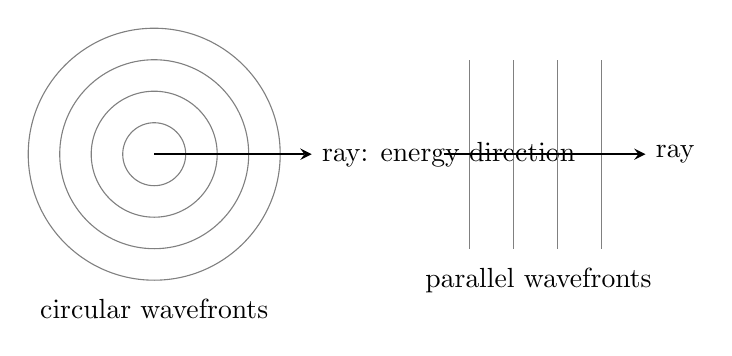
\begin{tikzpicture}[scale=.8,>=stealth]
\foreach \r in {.5,1,1.5,2}{\draw[gray] (0,0) circle (\r);}
\draw[->,thick] (0,0)--(2.5,0) node[right]{ray: energy direction};
\node at (0,-2.45){circular wavefronts};
\draw[gray] (5,-1.5)--(5,1.5); \draw[gray] (5.7,-1.5)--(5.7,1.5); \draw[gray] (6.4,-1.5)--(6.4,1.5); \draw[gray] (7.1,-1.5)--(7.1,1.5);
\draw[->,thick] (4.6,0)--(7.8,0) node[right]{ray}; \node at (6.1,-2){parallel wavefronts};
\end{tikzpicture}\end{center}
\smallskip

\begin{keybox}{Common trap}
A wavefront is not the wiggly line itself and a ray is not a physical ``beam edge''. They are models: wavefronts track phase; rays track energy direction. The perpendicular relationship is what makes them consistent.
\end{keybox}

\section{Light at materials}
A \textbf{luminous} object emits its own light: the Sun and a lit bulb are examples. A non-luminous object is seen only when light from another source reaches it and then reaches the eye.

A \textbf{transparent} material transmits most light; a little may be reflected. It is therefore possible to see an object through clear glass. An \textbf{opaque} material does not transmit light. It reflects some light and absorbs some. Saying simply ``opaque means black'' is wrong: a white wall is opaque but reflects a large fraction of the light falling on it.

\section{The law of reflection}
At a plane mirror, first draw the mirror. At the point where the incident ray hits, draw a dashed \textbf{normal}: an imaginary line at $90^\circ$ to the surface. Label the incoming ray as the incident ray and the outgoing one as the reflected ray. The angle of incidence $i$ is measured between the incident ray and the normal. The angle of reflection $r$ is measured between the reflected ray and the normal. The law is
\[\boxed{i=r}.\]

The most frequent examination error is measuring from the mirror surface. If a ray is $35^\circ$ to the normal, it is $55^\circ$ to the mirror, but the angle of incidence is $35^\circ$. The reflected ray must make $35^\circ$ on the other side of the normal. A check is symmetry: the two rays should look like a V reflected across the normal.

\begin{center}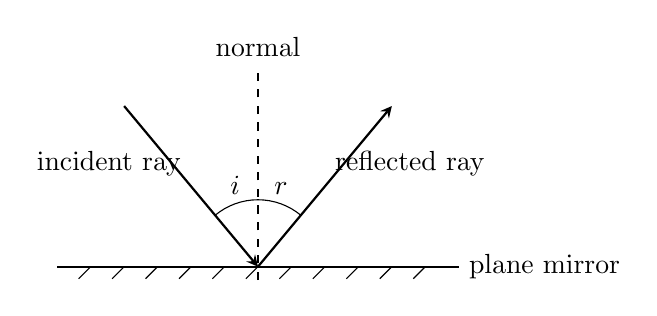
\begin{tikzpicture}[scale=.85,>=stealth]
\draw[thick] (-3,0)--(3,0) node[right]{plane mirror};
\foreach \x in {-2.5,-2,...,2.5}{\draw (\x,0)--(\x-.18,-.18);}
\draw[dashed] (0,-.2)--(0,3) node[above]{normal};
\draw[->,thick] (-2,2.4)--(0,0) node[midway,above left]{incident ray};
\draw[->,thick] (0,0)--(2,2.4) node[midway,above right]{reflected ray};
\draw (0,1) arc (90:130:1) node[midway,above]{$i$}; \draw (0,1) arc (90:50:1) node[midway,above]{$r$};
\end{tikzpicture}\end{center}

\begin{keybox}{Method for any reflection construction}
(1) locate the point of incidence; (2) draw the normal at $90^\circ$ to the local surface; (3) measure $i$ from the normal; (4) draw the reflected ray with the same angle on the other side; (5) add arrow directions and labels. On a curved surface the normal changes from point to point.
\end{keybox}

\section{Specular and diffuse reflection}
\textbf{Specular reflection} occurs at a smooth surface. Parallel incident rays meet parallel normals, so after reflection they remain parallel and travel in one direction. This is why a smooth mirror can make a clear image.

\textbf{Diffuse reflection} occurs at a rough surface. Each tiny patch still obeys $i=r$, but its normal points in a different direction from neighbouring patches. Parallel incident rays therefore leave in many directions. ``Diffuse'' does not mean that the law of reflection fails and it does not mean that the light is absorbed. It means the reflected directions are spread out, allowing a matte wall to be seen from many positions but not to form a sharp image.

\section{Curved reflectors and applications}
A funny mirror has a curved surface, so the local normal differs from place to place. Rays from different parts of a face are reflected by different amounts; their apparent origin is distorted, so the image looks stretched or squashed.

A satellite dish is shaped like a parabola. Parallel incoming radio waves reflect to one focal point. Bringing energy to the receiver at the focus concentrates a weak signal. A reflecting telescope uses a large concave mirror to collect light over a large area and focus it into a smaller area. A small plane mirror then directs the focused image towards the eyepiece. The concave mirror is not there merely ``to make light bounce''; its curvature gathers and focuses.

\section{Periscopes: use reverse ray tracing}
The lesson’s practical application was a periscope for seeing over a wall. Two plane mirrors are arranged parallel, commonly at $45^\circ$ to the tube. Light from the object reflects from the top mirror down the tube, then from the lower mirror into the observer’s eye. A robust drawing method is to start at the observer’s eye and work backwards: draw the final ray to the lower mirror, use $i=r$ to find its earlier direction, then repeat at the upper mirror until it reaches the object. Reverse construction is valid because light paths are reversible. It also prevents an attractive but useless diagram in which rays never enter the eye.

\section{Seeing, absorption and the visible band}
The lesson briefly used human vision as a way to think about the visible part of the spectrum. An object is visible only if light from it reaches the eye. A luminous lamp emits visible light directly. A non-luminous book is visible because it reflects some incident light. Its colour depends on which wavelengths are reflected more strongly and which are absorbed. This does not make visible light special in the physics of wave propagation: it is simply the narrow range to which human eyes respond.

Absorption is also a useful way to explain why a material can look different in different situations. If a material absorbs a particular wavelength, less of that wavelength emerges to the observer. Transparent materials transmit most of the relevant light, although they may reflect a little at each surface. Opaque materials transmit essentially none: incident light is divided between reflection and absorption. In an exam explanation, make the energy route explicit: incident light is reflected, absorbed or transmitted; then say which route reaches the observer.

Water featured in the discussion because absorption depends on wavelength. The safe GCSE conclusion is not that water “stops all waves”, but that a material may absorb some wavelengths more strongly than others. That is an interaction property of the material and the radiation. Avoid claiming that frequency changes merely because a wave is absorbed; frequency is set by the source. If a wave enters another medium, its speed and wavelength can change, but its frequency remains the same.

\begin{keybox}{Exam language: effect followed by mechanism}
For a medical X-ray, state that bone absorbs X-rays more than soft tissue, producing contrast at the detector. For a coloured object, state which wavelengths are reflected into the eye and which are absorbed. For transparency, state that light is transmitted. Naming a material without an interaction is usually too vague.
\end{keybox}

\section{Worked reasoning: reflection angles and wavefronts}
\textbf{Example 1.} A ray meets a horizontal plane mirror at $40^\circ$ to the mirror surface. Find the angle of incidence and the angle of reflection. The normal is perpendicular to the surface, so the angle between the incident ray and the normal is $90^\circ-40^\circ=50^\circ$. Thus $i=50^\circ$ and, by the law of reflection, $r=50^\circ$. The reflected ray is $40^\circ$ to the mirror surface on the opposite side. The common wrong answer is $40^\circ$: it has used the surface as the reference line.

\textbf{Example 2.} Plane wavefronts approach a vertical reflecting boundary from the left. Their rays are horizontal. Draw a normal at the point of incidence; because the boundary is vertical, this normal is horizontal. The reflected ray is constructed with equal angles around the normal. After reflection, the wavefronts must still be perpendicular to the reflected rays. This final perpendicularity check catches diagrams where a ray is correctly reflected but the wavefronts are copied without changing direction.

\textbf{Example 3.} Explain why a rough white wall can be seen from many places even though it is opaque. It is opaque, so light does not pass through it. It reflects a substantial fraction of incident visible light. Its rough surface gives different local normals, therefore the reflected rays leave in many directions. An observer in many positions can receive some reflected light. A white wall is not transparent; its appearance comes from diffuse reflection.

\textbf{Example 4.} Compare a plane mirror and a parabolic satellite dish. Both obey $i=r$ at every point. A plane mirror sends parallel incident rays into one parallel reflected direction. A parabolic dish has deliberately changing normals: parallel incoming waves are reflected to a focus. The application needs concentration at the receiver, which is why the dish shape matters.

\section{Exam-answer structure and misconceptions}
For a definition question, give the exact relationship first and then, if requested, an example. ``A normal is an imaginary line at 90 degrees to the surface at the point of incidence'' is much stronger than ``a line near the mirror''. For a comparison question, use paired language: smooth surface/parallel normals/parallel reflected rays versus rough surface/different normals/scattered reflected rays. This demonstrates cause and effect.

For an EM-spectrum order question, write all seven bands in one unambiguous sequence and attach the requested direction. If asked for an explanation of the order, invoke $c=f\lambda$ only after saying that all EM waves have the same speed in a vacuum. Do not say that gamma rays travel faster than radio waves in a vacuum: they have a higher frequency and shorter wavelength, not a higher vacuum speed.

For a radiation question, distinguish exposure from source. X-rays and gamma rays have useful applications, but their ionising nature means dose control is required. A chain such as ``gamma rays cause cancer because they are dangerous'' is circular. A chain such as ``gamma rays can ionise atoms in cells, which can mutate DNA and increase cancer risk'' earns the explanatory credit.

For a ray diagram, labels matter. Include incident ray, reflected ray, normal, angle of incidence and angle of reflection when the question asks for a construction. Use a ruler and ensure the normal passes through the point of incidence. In a periscope, ensure the final reflected ray reaches the eye; a diagram that has two equal-angle reflections but misses the eye does not answer the problem.

\section{A compact retrieval routine for this lesson}
Use a two-pass routine after the first read. First, write the EM spectrum from memory and annotate only three arrows: frequency up, wavelength down, energy up. Second, sketch a mirror with a normal and an arbitrary incident ray. Label $i$ from the normal, then construct $r$ without using a protractor. If either task feels slow, identify the missing relationship rather than merely rereading the answer.

For applications, practise explaining the same law in new contexts. Ask why a shiny spoon can make a recognisable image, why a painted wall cannot, why a curved fairground mirror distorts, and why a dish has a receiver at one point. Each answer begins with reflection, but the decisive detail is surface shape and therefore the pattern of normals. This is transferable reasoning, not a list of isolated facts.

\section*{Quick recall page}
\begin{tabularx}{\linewidth}{@{}p{.34\linewidth}X@{}}\toprule
Prompt & Answer to retrieve\\\midrule
Radio $\rightarrow$ gamma & frequency increases; wavelength decreases; energy increases.\\
Ionising danger & ionises atoms in cells $\rightarrow$ mutations $\rightarrow$ cancer risk.\\
Ray / wavefront & ray: energy direction; wavefront: equal phase; they are perpendicular.\\
Normal & imaginary line perpendicular to the surface at incidence.\\
Law of reflection & angles are measured from the normal and $i=r$.\\
Specular / diffuse & smooth: parallel rays leave parallel; rough: changing normals scatter rays.\\
Parabolic dish & parallel waves reflect to a focus, concentrating the signal.\\
Periscope & two reflections; trace backwards from the eye.\\\bottomrule
\end{tabularx}

\section*{Self-test}
1. Put microwave, ultraviolet, infrared and X-ray in ascending frequency.\\
2. Explain why an opaque white wall can be seen but cannot be seen through.\\
3. A ray is $28^\circ$ to a mirror surface. What are $i$ and $r$? Explain the reference line.\\
4. Why can diffuse reflection still obey the law of reflection?\\
5. Explain why a satellite dish has a focus.

\textit{Answers:} (1) microwave, infrared, ultraviolet, X-ray. (2) it reflects light to the eye but does not transmit it. (3) $i=r=62^\circ$, measured from the normal. (4) each local patch obeys $i=r$ relative to its own normal; the normals differ. (5) its parabolic shape reflects parallel incoming waves to one point, concentrating the signal.
\end{document}